\documentclass{article}[14pt,a4paper]
% Comment the following line to NOT allow the usage of umlauts
\usepackage[utf8]{inputenc}
%\usepackage[english]{babel}
\usepackage[legalpaper, lmargin=1.8cm, rmargin=1.8cm, bottom=1.8cm]{geometry}
\usepackage{color}
% Uncomment the following line to allow the usage of graphics (.png, .jpg)
\usepackage{verbatim}
\usepackage{graphicx}
\usepackage{amsmath}
\usepackage[all]{xy}
\usepackage{pst-all}
\usepackage{tikz}
\usepackage{lscape}
\usepackage{tikzpeople}
\usepackage{fancybox}
\usepackage{cancel}
%\usepackage{gnuplottex}
%\usepackage{chronology}
\usepackage{pst-pdf}
%\usepackage{pstricks}

\usepackage{pst-solides3d}
\usepackage{pgfplots}
\pgfplotsset{width=10cm,compat=1.9}
\pagestyle{empty}
 \usetikzlibrary{datavisualization.formats.functions} \usetikzlibrary{matrix.skeleton} \usetikzlibrary[shapes,arrows,positioning,fit,backgrounds,intersections,shadows,calc] \usetikzlibrary{positioning} \usetikzlibrary{decorations.text} \usetikzlibrary{decorations.pathmorphing}  \tikzset{flippedeventlabel/.append style={align=center}}
\usetikzlibrary{matrix.skeleton}
\usetikzlibrary[patterns,shapes,arrows,positioning,fit,backgrounds,intersections,shadows,calc]
\usetikzlibrary[datavisualization]
\usetikzlibrary{math}
% Start the document
\begin{document}
%\pagecolor{black}

%\tikz \datavisualization
%[scientific axes=clean,
%x axis={length=2.5cm, ticks={major at={
%5,
%6 as [style=red],
%7 as [{style=blue, low=-1em}],
%8 as [style=orange] $2^3$,
%10 as [style=magenta]ten
%}}},
%visualize as line]
%data [format=function] {
%var x : interval [5:10];
%func y = \value x * \value x;
%};\\
%\tikz \datavisualization
%[scientific axes,
%all axes={
%length=3cm,
%grid,
%grid={minor steps between steps}
%}, every major grid/.style = {style={blue, thin}},
%visualize as line]
%data [format=function] {
%var x : interval [5:10];
%func y = \value x * \value x;
%};\\
%Definiendo Paquete de Funciones 
\tikz \datavisualization data group {LogNormal} = {
data [set=log1, format=function] {
var x : interval [(0.1:5];
func y =(1/(0.3*sqrt(2*pi)*\value x))* exp(-(ln(\value x)-0)^2/(2*0.3^2);
}
data [set=log2, format=function] {
var x : interval [(0.1:5];
func y =(1/(0.5*sqrt(2*pi)*\value x))* exp(-(ln(\value x)-0)^2/(2*0.5^2);
}
data [set=log3, format=function] {
var x : interval [(0.1:5];
func y =(1/(0.7*sqrt(2*pi)*\value x))* exp(-(ln(\value x)-0)^2/(2*0.7^2);
}
};
\tikz \datavisualization data group {Dist Exponencial} = {
data [set=Exp1, format=function] {
var x : interval [0:5];
func y = 0.5* exp(-0.5*\value x);
}
data [set=Exp2, format=function] {
var x : interval [0:5];
func y =exp(-\value x);
}
data [set=Exp3, format=function] {
var x : interval [0:5];
func y =1.5*exp(-1.5*\value x);
}
data [set=linev1, format=function] {
var y : interval [0:0.18394];
func x = 2;
}
data [set=linev2, format=function] {
var y : interval [0:0.36788];
func x = 1;
}
data [set=linev3, format=function] {
var y : interval [0:0.55182];
func x = 0.66666;
}
};
\tikz \datavisualization data group {Acum Exponencial} = {
data [set=AExp1, format=function] {
var x : interval [0:5];
func y = 1- exp(-0.5*\value x);
}
data [set=AExp2, format=function] {
var x : interval [0:5];
func y =1-exp(-\value x);
}
data [set=AExp3, format=function] {
var x : interval [0:5];
func y =1-exp(-1.5*\value x);
}
};
\begin{center}
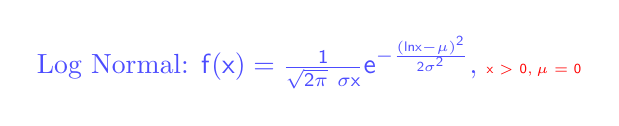
\begin{tikzpicture}
\draw node[blue!70]at (15,15) {Log Normal: $\mathsf{f(x) = \frac{1}{\sqrt{2\pi}\ \sigma x} e^{-\frac{(ln x-\mu)^2}{2\sigma^2}}}$,  \textcolor{red}{\tiny{$\mathsf{x > 0, \mu = 0}$}}};
\end{tikzpicture}\\
\tikz \datavisualization [scientific axes,
visualize as smooth line/.list=
{log1, log2, log3},
legend = south outside,
log1= {label in legend={text=$\sigma \to 0.3$}},
log2= {label in legend={text=$\sigma \to 0.5$}},
log3={label in legend={text=$\sigma \to 0.7$}},
style sheet=strong colors]
data group {LogNormal};

\vspace{0.5cm}
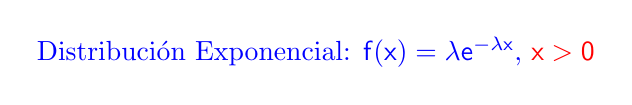
\begin{tikzpicture}
\draw node[blue]at (15,15) {Distribución Exponencial: $\mathsf{f(x) = \lambda e^{-\lambda x}}$,  \textcolor{red}{$\mathsf{x > 0}$}};
\end{tikzpicture}\\

\tikz \datavisualization
[scientific axes=clean,x axis={ticks={major at={
0 as [style=orange], 0.666 as [{style=blue, low=-1em}]$\frac{2}{3}$, 1 as [{style=red, low=-1em}], 2 as [{style=black, low=-1em}],
3 as [style=orange], 4 as [style=orange], 5 as [style=orange],}}},
visualize as smooth line/.list=
{Exp1, Exp2, Exp3, linev1, linev2, linev3},
legend = {south outside, label style = text colored},
Exp1= {label in legend={text=$\lambda\to 0.5 $}},
Exp2= {label in legend={text=$\lambda \to 1$}},
Exp3={label in legend={text=$\lambda \to 1.5$}},
style sheet = strong colors] 
data group {Dist Exponencial};\\

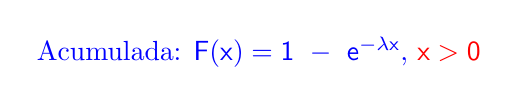
\begin{tikzpicture}

\draw node[blue]at (15,15) {Acumulada: $\mathsf{F(x) = 1\ -\  e^{-\lambda x}}$,  \textcolor{red}{$\mathsf{x > 0}$}};
\end{tikzpicture}\\

\tikz \datavisualization

[scientific axes,
visualize as smooth line/.list=
{AExp1, AExp2, AExp3},
legend = {south outside, label style = text colored},
AExp1= {label in legend={text=$\lambda\to 0.5 $}},
AExp2= {label in legend={text=$\lambda \to 1$}},
AExp3={label in legend={text=$\lambda \to 1.5$}}, style sheet = strong colors]
data group {Acum Exponencial};
\end{center}
\end{document}
